% Asset ID: FA22CentreOfMassTikZ-004
% Source: Phase 4 generated TikZ asset for FA22 Centre of Mass
% Related lesson section: Section 9 TikZ placeholders
% Purpose: Two-string suspension moment diagram.
\documentclass[tikz,border=8pt]{standalone}
\usepackage{amsmath}
\definecolor{Canvas}{HTML}{FAF9F6}
\definecolor{Ink}{HTML}{2C2C2E}
\definecolor{LineSoft}{HTML}{E5E5EA}
\definecolor{Gold}{HTML}{D4AF37}
\definecolor{Accent}{HTML}{C5A059}
\definecolor{Blush}{HTML}{FBEFEF}
\begin{document}
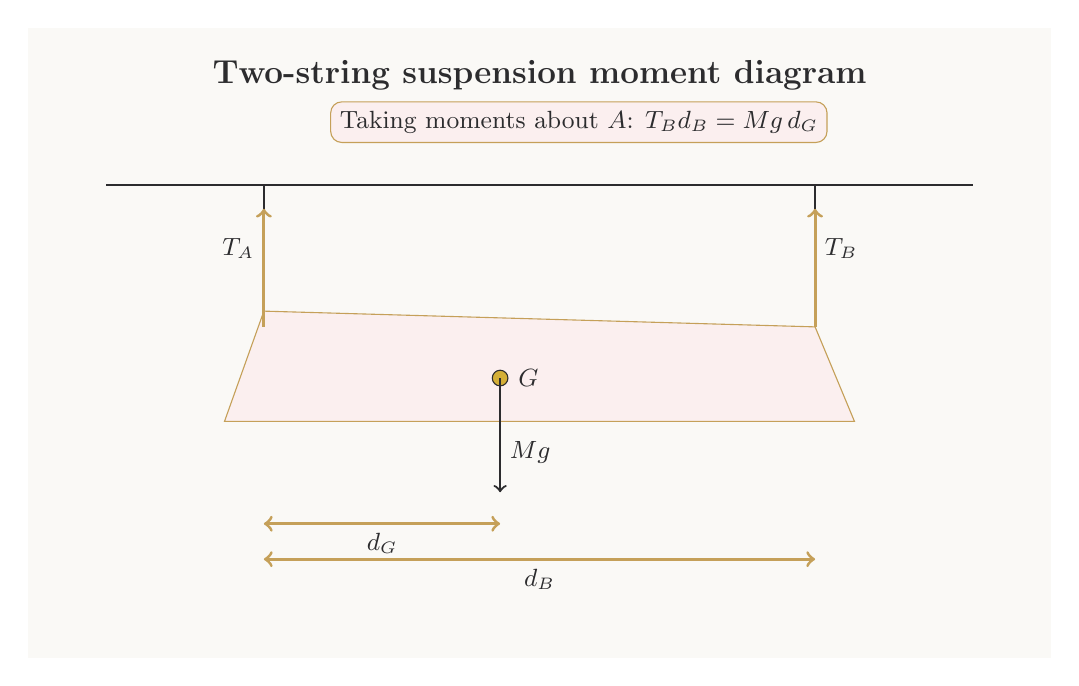
\begin{tikzpicture}[every node/.style={font=\small,text=Ink},line/.style={draw=Ink,line width=0.8pt},gold/.style={draw=Accent,line width=1.1pt},dot/.style={circle,fill=Gold,draw=Ink,inner sep=2pt}]
\fill[Canvas] (-1,-1) rectangle (12,7);
\node[font=\bfseries\large] at (5.5,6.4) {Two-string suspension moment diagram};

\draw[line] (0,5)--(11,5);\draw[line] (2,5)--(2,3);\draw[line] (9,5)--(9,3);
\draw[fill=Blush,draw=Accent] (1.5,2)--(9.5,2)--(9,3.2)--(2,3.4)--cycle;
\draw[->,gold] (2,3.2)--(2,4.7);\node[left] at (2,4.2){$T_A$};\draw[->,gold] (9,3.2)--(9,4.7);\node[right] at (9,4.2){$T_B$};
\node[circle,fill=Gold,draw=Ink,inner sep=2pt,label=right:{$G$}] at (5,2.55){};\draw[->,line] (5,2.55)--(5,1.1);\node[right] at (5,1.6){$Mg$};
\draw[<->,gold] (2,0.7)--(5,0.7);\node[below] at (3.5,0.7){$d_G$};\draw[<->,gold] (2,0.25)--(9,0.25);\node[below] at (5.5,0.25){$d_B$};
\node[draw=Accent,fill=Blush,rounded corners] at (6,5.8){Taking moments about $A$: $T_Bd_B=Mg\,d_G$};
\end{tikzpicture}
\end{document}
